\chapter{Related Work}
\paragraph{}
Generating base meshes from skeletons aids in modelling and rigging of more complex meshes. The most notable algorithms are B-Mesh\cite{ji_bm} by Ji et al. and Skeleton to Quad Dominant Mesh\cite{sqm} (SQM) by J. A. Bærentzen et al. This algorithms are capable of generating quad-dominant manifold meshes with good edge flow. Generated meshes are convenient because thanks to quad dominance and good edge flow they are easily skinned. Since the mesh is generated from skeleton we also implicitly know how much each bone affects vertices of the mesh during animation. We will also discuss some results from Michal Mc Donells master thesis Skeleton-based and interactive 3D modelling\cite{sqm_phd}. In particular the generation of capsule endings in SQM algorithm as we also wanted our algorithm to be capable of generating capsules.
\paragraph{}
B-Mesh algorithm and SQM algorithm present two different approaches to generation of base meshes from skeletons. B-Mesh algorithm firstly generates mesh for the limbs of the skeletons. These limb meshes are later joined together. On the other SQM algorithm firstly creates polyhedrons for branch nodes of the input skeleton. These polyhedrons are later joined with tubes consisting solely from quadrilaterals.
\paragraph{}
In this chapter we will describe both algorithms with their advantages and disadvantages. This serves to show why we have based our implementation on SQM algorithm.
\pagebreak

\section{B-Mesh algorithm}
\paragraph{Input}
B-Mesh algorithm takes as input a skeleton with a set of spheres or ellipsoids. Each node of the input skeleton has assigned a sphere or ellipsoid that represents its local geometry. Auxiliary spheres can be added to more precisely affect the resulting geometry of generated base mesh.
\paragraph{}
The algorithm consist of five steps:
\begin{enumerate}[\bfseries {Step} 1{:}]
	\itemsep-0.25em 
	\item Sphere generation - new spheres are generated along the bones of the skeleton.
	\item Sweeping - generation of mesh for skeletons limbs.
	\item Stitching - joining of limb meshes at branch nodes.
	\item B-Mesh evolution - subdivision and smoothing of generated mesh.
	\item B-Mesh fairing - fairing to improve edges flow.
\end{enumerate}
\begin{figure}[h]
    \centering
    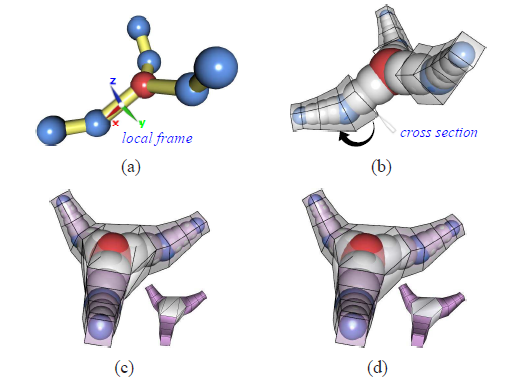
\includegraphics{images/b_mesh_ilu.png}
    \label{fig:b_mesh_stitch}
    \caption[B-Mesh sweeping and stitching illustration]{B-Mesh sweeping and stitching illustration. (a) local coordinates of a bone; (b) sweeping step; (c) stitching step; (d) after stitching simplification; Source \cite{ji_bm}}
\end{figure}

%\subsection{Sphere generation}
%\paragraph{}
\paragraph{Sphere generation}
Additional spheres are generated along the bones of the input skeleton. The distance between two spheres is defined by sampling step and the radius of each sphere is interpolated from radius's corresponding to the bones nodes. These generated spheres are used to refine the generated mesh and to calculate scalar field need in B-Mesh fairing step.

%\subsection{Sweeping}
%\paragraph{}
\paragraph{Sweeping}
For each bone its local coordinate system is generated as can be seen in Figure \ref{fig:b_mesh_stitch} (a). Limb mesh generation starts at branch nodes. For each new limb a rectangle aligned with limbs corresponding bones local axis is generated. Its points are then translated along the bones forming said limb and rotated around the connection nodes. After each translation the new points are connected with previous set of points in order to form a tube consisting of quadrilaterals. The resulting tubes can be seen in Figure \ref{fig:b_mesh_stitch} (b).

%\subsection{Stitching}
%\paragraph{}
\paragraph{Stitching}
Limb meshes generated in sweeping step are now stitched together. This is done by generating a convex hull from all the points corresponding to each branch nodes. These points are the beginning of each limb mesh tube. The result can be seen in Figure \ref{fig:b_mesh_stitch} (c). Generated convex hull is composed from triangles. To simplify them into quadrilaterals a score between each pair of triangles is computed. The score measures how close to a plane is each pair of triangles. The results of stitching simplification are shown in Figure \ref{fig:b_mesh_stitch} (d).

\paragraph{B-Mesh evolution}
Catmull-Clark subdivision is used to smooth the stitched mesh. However after smoothing the mesh shrinks and deviates from the spheres. A scalar field is generated and used to evolve the mesh. Each vertex of the stitched mesh is translated according to the scalar field and its evolution speed. This means the further away is the vertex from its corresponding sphere the more it is attracted to it. In this phase the auxiliary spheres are used to manipulate the scalar field and thus the final shape of the mesh. This step can be repeated multiple times to further smooth the mesh.

\paragraph{B-Mesh fairing}
After the evolution step certain edges may not be aligned with their principal directions. New vertex positions are calculated by iterative minimization of a function.

\paragraph{Conclusion}
The biggest problem with B-Mesh algorithm for our use is its iterative nature. The number of iterations is an input parameter and we wanted to avoid input parameters, so that the base mesh generation is as automatic as possible. Without the evolution step B-Mesh approximates input geometry worse than SQM. This is caused by the stitching phase which creates rectangular geometry at branch nodes, instead of the input spherical or elliptical geometry. Because of this evolution phase can not be avoided if we want to approximate the input as much as possible.
%\paragraph{}
B-Mesh algorithm is also running slower and produces more triangles than SQM according to \cite{sqm}. The auxiliary spheres and ellipsoid nodes are interesting additions that were not present in SQM. But we wanted to modify the generated base mesh geometry directly on GPU during rendering so they are not advantageous to our intended use. B-mesh algorithm can generate capsules but it needs several evolution steps to precisely match capsules geometry. The algorithm looks like it can be naturally extended to support cyclic skeletons. Sweeping steps occurs only on limb paths and stitching occurs directly at branch nodes. Evolution and fairing moves vertices directly so it is independent from cycles in the input skeleton.

\section{Skeleton to Quad Dominant Mesh algorithm}
\paragraph{Input}
The input to SQM algorithm is a skeleton. Similarly to B-mesh for each of skeletons nodes a sphere is defined to represent local geometry. Contrary to B-mesh algorithm SQM does not support ellipsoid nodes. SQM algorithm has also an extra limitation that the root of the skeleton has to be a branch node.
\paragraph{}
The algorithm consist of four steps and one preprocessing step:\\
\textbf{Preprocessing:} Skeleton straightening - serves to simplify step number 3 of the algorithm.
\begin{enumerate}[\bfseries {Step} 1{:}]
	\itemsep-0.25em 
	\item BNP generation - generation of branch node polyhedrons (BNPs).
	\item BNP refinement - subdivisions of BNPs.
	\item Creating the tubular structure - bridging of BNPs.
	\item Vertex placement - reverting straightened mesh to its original pose.
\end{enumerate}

\begin{figure}[h]
    \centering
    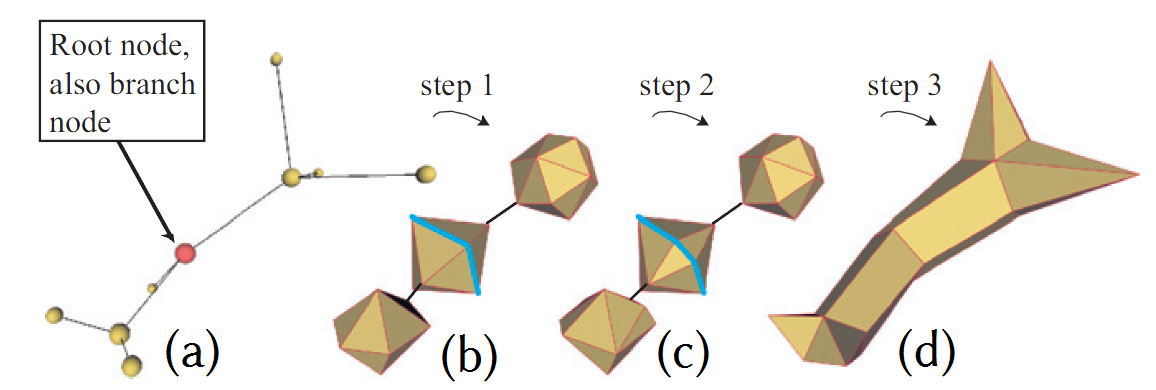
\includegraphics[width=\textwidth]{images/sqm_viz.png}
    \label{fig:sqm_algorithm_steps}
    \caption[Steps of SQM algorithm]{Steps of SQM algorithm. (a) the input skeleton; (b) generated BNPs; (c) refined BNPs; (d) BNPs bridges with quadrilateral tubes; Source \cite{sqm}}
\end{figure}

\paragraph{Skeleton straightening}
This is a preprocessing step of the algorithm that simplifies the generation of tubular structures. For each connection node its child is rotated, so that the edge between connection node and its child is parallel with the edge between connection node and its parent. This is usefully because during step 3 the algorithm needs to only generate straight tubes and does not need to take rotation into account.

\paragraph{BNP generation}
A branch node polyhedron(BNP) is a polyhedron assigned to a branch node. Vertices of a BNP correspond to a set of points that are generated by intersecting the sphere assigned to a branch node with each edge connected to said branch node. We will call this vertices intersection vertices. To form a BNP intersection vertices are triangulated. After that each triangle is split into six triangles by inserting one vertex in the middle of each triangle and in the middle of each of the edges of the triangle. These vertices are then projected back onto the sphere associated with a branch node. This projection is needed because if the intersection vertices are coplanar the generated polyhedron would have no volume. The result of this step can be seen in Figure \ref{fig:sqm_algorithm_steps} (b).

\paragraph{BNP refinement}
During step 3 of the algorithm BNPs connected via path are bridged with tubes consisting solely from quadrilaterals. This is done be connecting the one-rings of two corresponding intersection vertices with faces. To ensure that we can use only quadrilaterals the one-rings need to have the same valency. So each BNP is refined so that the valency of two intersection nodes lying on the same path are equal. This can be seen in Figure \ref{fig:sqm_algorithm_steps} (c).

\paragraph{Creating the tubular structure}
After previous step of the algorithm connected BNPs can be joined by a tube formed by quadrilaterals. The tube is divided into segments. Each of the segments corresponds to a connection node. Vertices corresponding to a certain connection node are projected onto its corresponding sphere. Leaf nodes are terminated with a triangle which central vertex corresponds to the leaf nodes vertex. The result is illustrated in Figure \ref{fig:sqm_algorithm_steps} (d).

\paragraph{Vertex placement}
The base mesh is now finished. All that remains is to reverse the rotations used to straighten the input skeleton. After final vertex placement the resulting mesh is smoothed using with three iterations of Laplacian smoothing and attraction scheme.

\paragraph{Conclusion}
Each of SQMs steps are one pass algorithms except the final smoothing and attraction scheme application. But since SQM generates branch node geometry by generating a polyhedron it better resembles the geometry of the input skeleton even without smoothing. Cyclic meshes can be problematic to implement, because in the refinement step of the algorithm a cyclic mesh may cause an infinite loop of refining. SQM produces smaller number of triangles because in the joining phase all triangles corresponding to branch nodes are removed and their former vertices are used to generate connecting tubes. On the other hand during the stitching phase B-Mesh introduces triangles into the mesh. SQM algorithm was also capable of generating cycles from two symmetric leaf node,s that were close to each other. However these cycles can not be created explicitly. Another limitation is that cycles have to lie on input skeletons axis of symmetry.

\section{Skeleton-based and interactive 3D modelling} 
\paragraph{}
Michal Mc Donells master thesis studies the capabilities of SQM algorithm. It aims to extend SQM algorithm through pre-processing of SQMs input skeleton and post-processing of the output mesh. Altering SQM algorithm itself was out of scope of the thesis. Among the improvements to the algorithm were cone, cube, sphere and hemisphere leaf nodes, cube connection and branch nodes as well as concavities and branch node root requirement. The most important parts for us are spherical leaf nodes and branch node root requirement.

\begin{figure}[h]
    \centering
    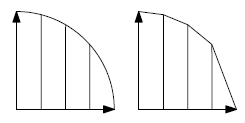
\includegraphics[]{images/spherical_node.png}
    \label{fig:esqm_spherical}
    \caption[Spherical nodes radii]{Left: arc subdivided at fixed intervals; Right: radii of newly inserted nodes sampled from an arc on the left; Source \cite{sqm_phd}}
\end{figure}

\paragraph{Spherical leaf node}
Original SQM algorithm was not able to create spheres at leaf nodes. This also limited its ability to generate capsules that we wanted to implement in our algorithm. In the thesis a solution was presented that a spherical node would be represented by several connection nodes. The first connection node would have the same radius as the desired sphere and each subsequent node would have its radius decreased until the desired number of subdivisions would be reached. We can see the process in Figure \ref{fig:esqm_spherical}. An arc with equal radius as the original spherical node would be sampled at fixed intervals. With enough samples the resulting mesh would approximate a sphere. However in the original SQM algorithm after Laplacian smoothing the smoothed mesh did not approximate the input sphere.

\paragraph{Conclusion}
The approach to create spherical nodes presented in the thesis seems suitable for our needs. Since we would not implement Laplacian smoothing we would not have problems with deformation of the generated sphere. On the contrary this approach is beneficial to our needs, since we wanted to smooth the generated mesh in tessellation shaders and keeping spherical meshes generated without post-processing can potentially ease the work-flow.

\paragraph{Root branch node requirement}
One of the limitations of SQM algorithm is that the root node has to be a branch node. The proposed solution to this limitation was to generate pseudo paths from the root to ensure that it always will have at least three child nodes. For example, if the root has only two childes the new node would be generated in a direction perpendicular to a line connecting the intersection of roots associated sphere and edges from root to its childes.

\paragraph{Conclusion}
This pseudo path generation would disturb the edge flow as it would introduce new unnecessary edges. We believe that a better approach would be to re-root the tree and replace its former root with a node with at least three childes. Linear skeletons without branching and skeletons consisting only from a single node would become special cases that would be handled separately. This would allow us to avoid the requirement without altering the expected edge flow of the input skeleton.